\documentclass[12pt, twoside]{article}
\usepackage[letterpaper, margin=1in, headsep=0.5in]{geometry}
\usepackage[english]{babel}
\usepackage[utf8]{inputenc}
\usepackage{amsmath}
\usepackage{amsfonts}
\usepackage{amssymb}
\usepackage{tikz}
\usetikzlibrary{quotes, angles}
\usepackage{graphicx}
\usepackage{enumitem}
\usepackage{multicol}

\newif\ifmeta
\metatrue %print standards and topics tags

\title{Regents Geometry}
\author{Chris Huson}
\date{September 2020}

\usepackage{fancyhdr}
\pagestyle{fancy}
\fancyhf{}
\renewcommand{\headrulewidth}{0pt} % disable the underline of the header
\raggedbottom


\fancyhead[LE]{\thepage}
\fancyhead[RO]{\thepage \\ Name: \hspace{4cm} \,\\}
\fancyhead[LO]{BECA / Dr. Huson / Geometry 02-Midpoint+distance\\* pset ID: 28}

\begin{document}

\subsubsection*{2-7DN-Compound-areas+perimeters}
\begin{enumerate}
\item Find the area $A$ and perimeter $P$ of a square with sides of length 10 centimeters. \vspace{4cm}
    
\item Find the area $A$ and perimeter $P$ of the shape shown below. The grid is in centimeters.
    \begin{flushleft}
      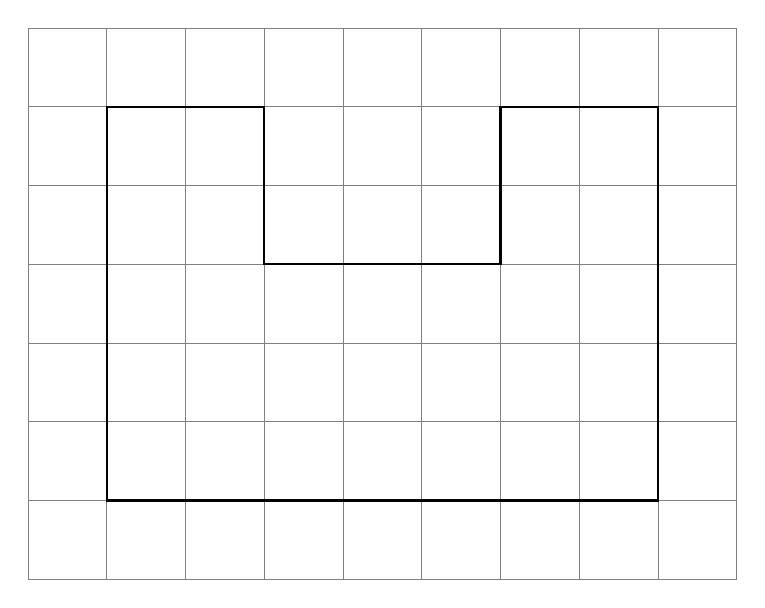
\begin{tikzpicture}[scale=1]
        \draw [help lines] (-4,-4) grid (5,3);
        %\draw [thick, ->] (-2.2,0) -- (10.4,0) node [below right] {$x$};
        %\draw [thick, ->] (0,-2.2)--(0,10.4) node [left] {$y$};
        %\draw (0,0) circle [radius=3] node[below]{$C$};
        %\draw [fill] (0,0) circle [radius=0.05];
        \draw [thick, -] (-3,-3)--(4,-3)--(4,2)--(2,2)--(2,0)--(-1,0)--(-1,2)--(-3,2)--cycle;
      \end{tikzpicture}
    \end{flushleft}
      
\item The area of a square is 100 square centimeters. Find the length of the side of the square. \vspace{3cm}
    
\item The perimeter of a square is 100 square centimeters. Find the length of the side of the square.

    \newpage


\item On the grid below, accurately draw and label two adjacent squares, one with a side length of 4 cm, the other with a side length of 3 cm. The grid is in centimeters.\\*[5pt]
    Find the area $A$ and perimeter $P$ of combined shape.
    \begin{flushleft}
      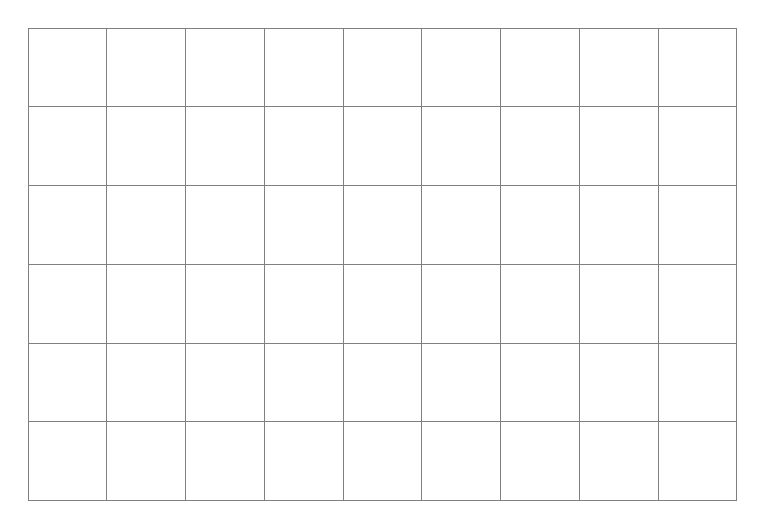
\begin{tikzpicture}[scale=1]
        \draw [help lines] (-4,-3) grid (5,3);
        %\draw [thick, ->] (-2.2,0) -- (10.4,0) node [below right] {$x$};
        %\draw [thick, ->] (0,-2.2)--(0,10.4) node [left] {$y$};
        %\draw (0,0) circle [radius=3] node[below]{$C$};
        %\draw [fill] (0,0) circle [radius=0.05];
        %\draw [thick, -] (-3,-3)--(4,-3);
      \end{tikzpicture}
    \end{flushleft} \vspace{1cm} 

\item Find the area of shape $ABCDE$ below, a triangle on a rectangle. The altitude $h$ of the triangle is $3 \frac{1}{2}$ centimeters and the base $AB=5 \frac{1}{2}$ cm. The rectangle is 1 cm tall. (diagram not to scale) \\[0.5cm]
      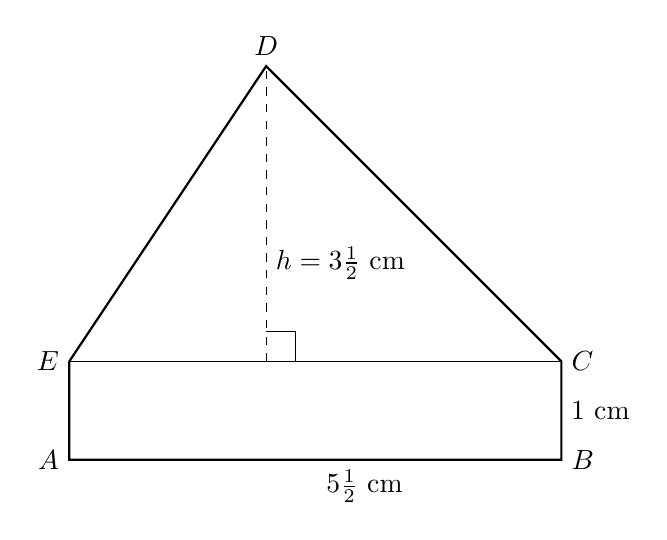
\begin{tikzpicture}[scale=1.25]
        \draw (2,0)--(7,0);
        \draw [thick] 
          (2,0)node[left]{$E$}--
          (2,-1)node[left]{$A$}--
          (7,-1)node[right]{$B$}--
          (7,0)node[right]{$C$}--
          (4,3)node[above]{$D$}--(2,0);
        \draw [dashed] (4,0)--(4,3);
        \draw (4,0)++(0.3,0)--++(0,0.3)--+(-0.3,0);
        \node at (4,1)[right]{$h=3 \frac{1}{2}$ cm};
        \node at (5,-1)[below]{$5 \frac{1}{2}$ cm};
        \node at (7,-0.5)[right]{$1$ cm};
      \end{tikzpicture} \vspace{1.0cm}

   
\end{enumerate}
\end{document}